\documentclass[10pt]{IEEEtran}
\usepackage[numbib]{tocbibind}
\usepackage{graphics}
\usepackage{caption}
\usepackage{subcaption}
\usepackage{graphicx}
\usepackage{authblk}

\graphicspath{ {./images/} }
\bibliographystyle{IEEEtran}

\title{
    Wine Not? \\
    \large An exploration into the language of wine reviews
}
\author[1]{Austin Doolittle}
\author[1]{Maria Corina Cabezas}
\affil[1]{University of California, Berkeley, \authorcr Email: {\tt \{austin.doolittle, m.cabezas95\}@berkeley.edu}\vspace{1.5ex}}

\begin{document}
\maketitle
\begin{abstract}
    WAIT TO DO THIS AFTER THE REMAINDER OF THE REPORT IS COMPLETE
    This is our abstract. Here we'll give a high level overview of what is was that we set out to accomplish and give a nseak preview of our results.
\end{abstract}

\section{Introduction}
    Understanding user reviews is an essential part of any product branding and marketing strategy. Reviews can also provide companies with important feedback about the product and assist decision making. Our goal is to use Natural Language Processing algorithms to automate the process of analyzing wine reviews. We'll train a regression model that predicts the price of the wine and the score given to the wine by professional reviewers. We'll also break down the score into a classification task, creating a psuedo-sentiment analysis model. This sentiment analysis model is particularly useful for wine companies trying to understand their own product reviews and see what blends are triggering more positive responses. 

\section{Background}
    We intend to perform experiments with a wide array of different Natural Language Processing algorithms to achieve our goal of understanding the luxury wine market via professional reviews. In order to determine which algorithms will be effective at this task, we should first identify the source and purpose of the dataset, then qualify the algorithms we intend to use with the problems that they solve.

\subsection{The Dataset}
    The dataset consists on 130,000 wine reviews scraped for the WineEnthusiast magazine in November, 2017. It includes the wine name, variety, name and location of the winery, price, and the review text and score. The dataset and scraping algorithm are retrieved from Kaggle\cite{data}. \par
    Official wine scoring is done on a scale from 50 to 100, with a higher score indicating that the wine is superior\cite{wine_scoring}. WineEnthusiast will not publish reviews for any wine that scores less than 80 points, so the range of possible values for this specific dataset is 80 to 100. \par
    We should be mindful that there are 19 reviewers in our dataset, with one reviewer amounting for 1/10 of all reviews. This might indicate the dataset is not representative of the market itself, and we should be mindful of this bias when drawing conclusions from the data. 
    Also, the dataset is not balanced in the number of reviews per each wine variety and region, with most reviewed wines coming from the United States and being Cabernet Sauvignon. View Figure \ref{data_distributions} for more information regarding the distributions of different values in the dataset. \par

    \begin{figure} % TODO fix graph alignment
    \centering
    \begin{subfigure}[t]{0.4\textwidth}
        \centering
        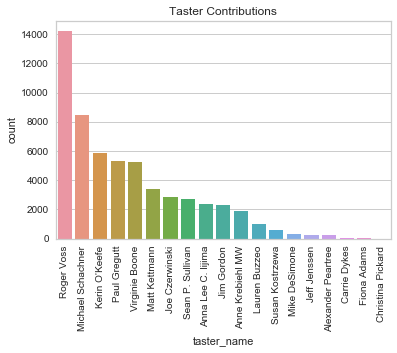
\includegraphics[width=\textwidth]{taster_contribution}
        \caption{Taster contributions plotted}
    \end{subfigure}
    \begin{subfigure}[t]{0.4\textwidth}
        \centering
        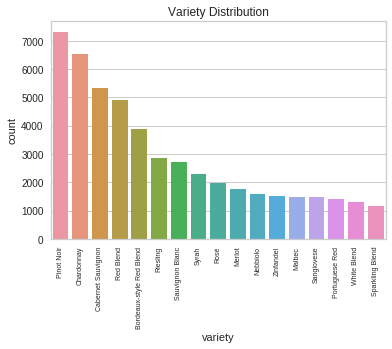
\includegraphics[width=\textwidth]{variety_distribution}
        \caption{Varieties with counts >1000 plotted}
    \end{subfigure}
    \caption{Distributions of different labels in the dataset}
    \label{data_distributions}
    \end{figure}

    Research in the NLP field has also shown that some difficult benchmark datasets contain latent bias that allow more complex models to perform very well on those tasks. One example of research that identified this bias found that it was easily identifiable by observing the presence or absence of specific words in relation to their labels\cite{clever_hans}. In an attempt to identify this bias before our analysis, we conducted Pearson correlation studies on all unigrams, bigrams, and trigrams in our dataset. Figure \ref{correlations} displays the correlations between unigrams and the price and score labels. We show here that we found no significant correlation on either end of the spectrum, and also observed symmetry between positive and negative correlations of ngrams in the corpus. This soothed fears of a biased dataset in this regard, and allowed the experiments to continue without major intervention.
    \footnote{More analysis was done in our preliminary investigation of this dataset than what is included in this section. Those results are included in the appendix for brevity} \par

    \begin{figure}
    \centering
    \begin{subfigure}[t]{0.4\columnwidth}
    \begin{tabular}{ |l||r| }
        \hline
        Unigram & $r_{price}$ \\
        \hline
        \hline
    \end{tabular}
    \caption{Correlations of unigrams with price}
    \end{subfigure}
    \begin{subfigure}[t]{0.4\columnwidth}
        \begin{tabular}{ |l||r| }
            \hline
            Unigram & $r_{score}$ \\
            \hline
            \hline
        \end{tabular}
        \caption{Correlations of unigrams with review score}
        \end{subfigure}
    \caption{Observations of correlations between Unigrams and their labels}
    \end{figure}

    
\subsection{Regression}
    In many cases, Linear Regression is able to solve regression problems with low error. While this is typically not the case for problems as complex as natural language processing, we will include it in our analysis to ensure we don't use too powerful of a model for our task. Linear Regression requires a feature set. For this, we can look to the age-old Bag-of-Words approach\cite{bag_of_words}. This approach is computationally simple, but only achieves that simplicity with some assumptions. Spatial relationships from the source text are not retained, thus forcing the assumption that the position of a token is not dependent on the outcome variable.\par
    Research has also shown that CNNs are capable of learning more complex relationships within blocks of text with the advantage of maintaining spatial relationships between tokens in the text\cite{cnn}. We intend to use a simple CNN for regression tasks, as 
    


\section{Exploratory Data Analysis}
    Here we outline some insights that we found in our exploration of the dataset. All graphs are visualized with the python library seaborn \cite{seaborn}, and the wordcloud was generated with the python library wordcloud \cite{wordcloud}

\subsection{Vocabulary}
    We now inspect the frequency of words in the dataset to identify any outliers, or high correlations between tokens and their labels.

    \begin{figure}
    \centering
    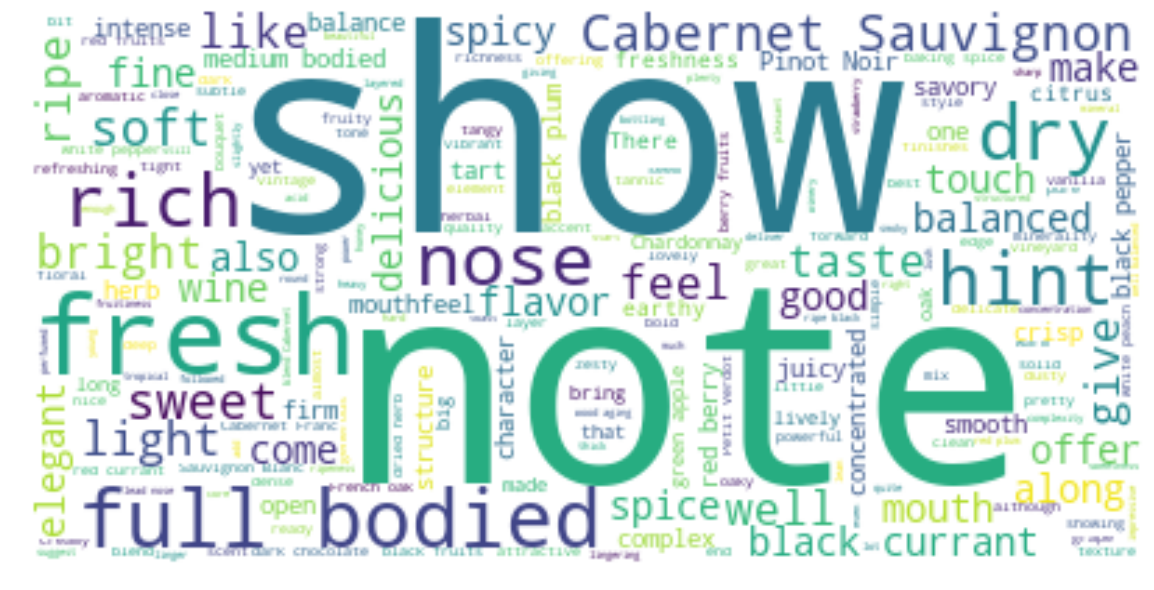
\includegraphics[width=\columnwidth]{wordcloud}
    \caption{Word cloud of the dataset's vocabulary}
    \end{figure}

    Notes from Meeting 11/26:
    - include distribution of scores and prices - Maria
        - touch on log-price, which is standard for currency based analysis
    - Include taster, region, variety graphics in disclaimer in dataset section - Maria
    - taster vocab in appendix - Austin
    - unigram correlations were an attempt to identify high correlation between points and score, refrence https://thegradient.pub/nlps-clever-hans-moment-has-arrived/ - Maria

\section{Approach}
    As mentioned above, we set out to perform regression on the score and price of the wine, classification on the region and variety of wine, and sentiment analysis. The following outlines the approachs that we take for each of these problems.

\subsection{Regression}
    We used three different types of models in our regression analysis. Prior to these expiriments we split the data randomly into a train, test, and validation set. The sizes of these datasets are 71973, 23991, and 23991, respectively. We preprocessed our text by removing all stop words, which in our implementation were a combination of NLTK's stopword collection, punctuation, and the top 10 most common words in the training dataset. We used Mean Squared Error as both a loss function and an evaluation metric for all models. We normalize the score of the wine by scaling the values so the mean of the distribution is 0 and standard deviation is 1. We also take the base 10 log of the price and regress on that value. \par
    The first was the SKLearn implementation of Linear Regression with a Bag-of-Words feature vector as input. The words were tokenized via the SKLearn $CountVectorizer$, with all words being lowercased, split on spaces, and combined into ngrams of varying sizes, each of which are evaluated and shown in the results section. \par
    The next model is a CNN model. The model was implemented in Keras \cite{keras}, an consists of an embedding layer which creates an embedding of size 256, followed by 3 parallel convolutional layers with filter sizes of 3, 4, and 5. The output of those layers are concatenated and fed as input into a fully connected layer, with dropout of probability 0.1. The output of the model is a single scalar value that does not have an activation function. The text is preprocessed and tokenized with the Keras preprocessing library. \\
    Finally, our last model is a keras implementation of BERT. The implementation was found on GitHub and is authored by CyberZHG\cite{keras_bert}. Our BERT Model has 12 transformers with 4 attention heads, a fully connected layer of size 100, and an embedding layer creating word vectors of size 256. The fully connected layers also have droupout applied with probability 0.05.

\subsection{Classification}
AUSTIN

\subsection{Sentiment Analysis}
    MARIA
    The goal is to conduct a sentiment analysis on wine reviews. The trained model is useful for wine companies trying to predict sentiment on new or existing products by looking at the specific aspects that are generating positive/negative emotions on people.   
    To approach this problem we will be using Natural Language Processing techniques, like Bag of Words (BoW) model and Word2Vec model to convert text into numerical representations. Then we fit the numerical representations to machine learning algorithms like Multinomial Naive Bayes, Logistic Regression and Random Forest. 
    The first step is to convert reviews into numerical representations using count vectorizer. Then we will train a Multinomial Naive Bayes Classifier and evaluate using accuracy score, precision, recall and f1-score. 
    INSERT ACCURACY AND CLASSIFICATION REPORT HERE.
    Instead of using occurance counting, we can use tf-idf vectorizer to scale down the impact of frequenty appeared words in a given corpus. Then we train a Logistic Regression and evaluate using accuracy score, precision, recall and f1-score. 
    INSERT ACCURACY AND CLASSIFICAION REPORT HERE. 
    Here we train a Word2Vec model to create our own word vector representations using the gensim library. Then we fit the feature vectors of the reviews to a Random Forest classifier. Finally we evaluate the model using accuracy socre, precision, recall and f1-score. 
    INSERT ACCURACY AND CLASSIFICATION REPORT HERE. 

\section{Results}
    We will now disclose the results of our expiriments in Regression, Classification, and Sentiment Analysis.

\subsection{Regression}
    Figure \ref{regression_results} contains a table of the Mean Squared Error achieved by all models the regression task for both wine score and log-price. The BERT model performed best on the score regression task, however the CNN was very close behind. We also note that unigram Bag-of-Words with a Linear Regressor performed best of all the linear models. We expect this to be a result of the size of the dataset. There are many unique bigrams and trigrams in the dataset, which likely causes overtraining. For the wine price model, we similarly see that the BERT and CNN models performed best, but in this case the CNN edged ahead of the BERT model. We see a similar pattern here in regards to the ngram size, which supports our hypothesis.

    \begin{figure}
    \centering
    \resizebox{\columnwidth}{!}{%
    \begin{tabular}{ |l||r|r|  }
        \hline
        \multicolumn{3}{|c|}{Regression Results} \\
        \hline
        Model& Review Score (MSE) & Wine Price (MSE) \\
        \hline
        $Linear BoW_{unigram}$   & 0.325          & 0.546 \\
        $Linear BoW_{bigram}$    & 0.647          & 0.809 \\
        $Linear BoW_{trigram}$   & 0.901          & 0.901 \\
        $Linear BoW_{1-3gram}$   & 0.460          & 0.805 \\
        \hline
        $CNN$                    & 0.285          & \textbf{0.499} \\
        \hline
        $BERT$                   & \textbf{0.283} & 0.513 \\
        \hline
    \end{tabular}}
    \caption{ Results of various regression models applied to the dataset. }
    \label{regression_results}
    \end{figure}

\subsection{Sentiment Analysis}
    MARIA
    This is where our sentiment analysis results should go

\section{Conclusion}
    BOTH
    This is where we should sum up our research in a paragraph or two

\newpage
\newpage
\bibliography{final_report}

\newpage
\section{Appendix}

\subsection{Stop Words}
TODO format this as a table
["your", "weren", "don", "having", "before", "finish", "didn", "(", "in", "does", "d", "you'll", "needn", "yourself", "what", "under", "than", ";", "\~", "any", "nor", "from", "why", "needn't", "weren't", "both", "up", "further", "during", "there", "them", "at", "wasn't", "same", "s", "<", "just", "below", "it", "again", "didn't", "aromas", "those", "haven", "ma", "now", "mustn't", "if", "itself", "him", "has", "no", "|", "which", "our", "was", "i", "such", "drink", "for", "can", "o", "over", "how", "with", "this", "my", "be", "ll", "\textbackslash", "`", "yourselves", "aren't", "once", "hadn't", "after", "you", "do", "here", "\&", "me", "where", "about", "don't", "by", "flavors", "then", "themselves", "own", "hadn", "hers", "doesn", "her", ".", "is", "?", "down", "tannins", "wouldn", "[", "of", "aren", "been", "or", "y", "few", "shouldn", "through", ":", "between", "who", "have", "mightn't", "/", "isn", "it's", "when", "he", "and", "against", "an", "herself", "ve", "=", "+", "]", "\{", "very", "a", "couldn't", "wasn", "t", "wouldn't", "\#", ")", "their", "out", "\_", "but", "because", "ain", "won", "yours", "couldn", "shouldn't", "\^", "these", "isn't", "they", "into", "myself", "were", "m", "shan", "only", "all", "his", "that'll", "had", "she's", "as", "haven't", ">", "its", "so", "cherry", "more", "too", "each", "did", "\$", "she", "ourselves", "am", "should've", "whom", "you're", "doing", "shan't", "*", "are", "the", "until", "himself", "being", "you'd", "other", "will", "mustn", "\%", "re", "that", "-", "we", "you've", "not", "acidity", "won't", "mightn", """, "ours", "doesn't", "\}", "above", "!", "some", "while", "'", "fruit", "wine", "@", "hasn", "most", "to", "on", ",", "off", "should", "hasn't", "palate", "theirs"]



\subsection{NGram Top Counts}
\begin{figure}
    \centering
    \begin{subfigure}[t]{\columnwidth}
        \centering
        \begin{tabular}{ lr  }
            \hline
            Unigram & Count \\
            \hline
            black  & 15967 \\
            ripe   & 14979 \\
            red    & 11949 \\
            spice  & 10658 \\
            notes  & 10438
        \end{tabular}
        \caption{ Top five unigram counts}
    \end{subfigure}
    \begin{subfigure}[t]{\columnwidth}
        \centering
        \begin{tabular}{ lr  }
            \hline
            Bigram & Count \\
            \hline
            full bodied & 3786 \\
            cabernet sauvignon & 2931 \\
            medium bodied & 1794 \\
            pinot noir & 1757 \\
            red berry & 1710
        \end{tabular}
        \caption{ Top five bigram counts}
    \end{subfigure}
    \begin{subfigure}[t]{\columnwidth}
        \centering
        \begin{tabular}{ lr  }
            \hline
            Trigram & Count \\
            \hline
            new french oak  & 436 \\
            red berry fruits & 381 \\
            blend cabernet sauvignon & 322 \\
            cabernet sauvignon merlot & 309 \\
            merlot cabernet sauvignon & 228 
        \end{tabular}
        \caption{ Top five trigram counts}
    \end{subfigure}
    \caption{1-3gram top counts}
    \end{figure}
\end{document}
